\chapter{Applications et morphismes}
\begin{abstract}
Au chapitre précédent, des espaces ont été définis, mais on ne s'est pas
intéressé beaucoup aux relations entre eux ou au sein d'eux.

Des distances, normes... ont été introduites, sans utiliser plus que ça le
vocable de fonction. Le terme d'injection a été prononcé à la fin du
chapitre précédent comme fil conducteur pour introduire celui-ci...

Dans ce chapitre, nous ne présenterons pour le coup que des choses extrêmement
«rudimentaires» et toutes vues en taupe ou avant. Il s'agit uniquement d'un aide-mémoire.
%
%\medskip
%Pour la bibliographie, nous nous référerons comme d'habitude à:\\
%\indent --
%Laurent \textsc{Schwartz}, \emph{Analyse I: Théorie des ensembles et Topologie},
%Hermann, 1992.\\
%Et pour tout savoir sur les opérateurs, on pourra compléter la lecture par:\\
%\indent --
%Tosio \textsc{Kato}, \emph{Perturbation Theory for Linear Operators}, Classics in Mathematics, Springer,
%1995 (reprint de 1980)
\end{abstract}


%\medskip
\begin{histoire}%
L'univers mathématiques du début du \textsc{xviii}\fup{e} siècle est dominé par Leonhard Euler\index[aut]{Euler (Leonhard Paul), 1707-1783, Suisse}
et par ses apports tant sur les fonctions que sur la théorie des nombres, tandis que Joseph-Louis
Lagrange\index[aut]{Lagrange (Joseph Louis, comte de -), 1736-1813, Italien}
 éclairera la seconde moitié de ce siècle.

%Au chapitre précédent, nous avons mentionné les travaux d'Euler sur les infinitésimaux,
%le calcul différentiel et intégral.
\sbox{\MaBoiteAvecPhotos}{\setlength{\tabcolsep}{0pt}\scriptsize%
\begin{tabular}{cccc}%
\includegraphics[height=\the\HauteurDesPhotos]{Euler2}&%
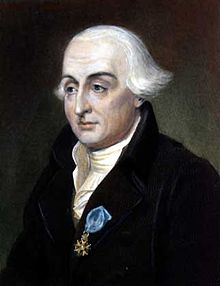
\includegraphics[height=\the\HauteurDesPhotos]{Lagrange}&%
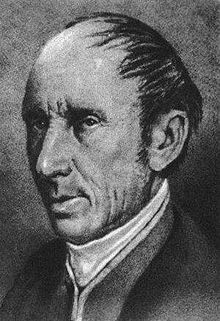
\includegraphics[height=\the\HauteurDesPhotos]{Cauchy2}&%
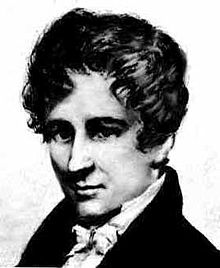
\includegraphics[height=\the\HauteurDesPhotos]{Abel}\\%
Euler &Lagrange &Cauchy &Abel%
\end{tabular}}
\medskip
\ImageADroite{%
Euler a introduit et popularisé plusieurs conventions de notation par le biais de ses nombreux ouvrages
largement diffusés.
Plus particulièrement, il a introduit la notion de fonction (dans L'\emph{Introductio in analysin infinitorum},
premier traité dans lequel le concept de fonction est à la base de la construction mathématique, et dont
les premiers chapitres lui sont consacrés) et a été le premier à écrire~$f(x)$
pour désigner la fonction~$f$ appliquée à l'argument~$x$, en 1734 (bien que le terme
de «fonction» apparaisse pour la première fois dans un manuscrit d'août 1673
de Leibniz,\index[aut]{Leibniz (Gottfried Wilhelm), 1646-1716, Allemand}
resté inédit, et intitulé \emph{la Méthode inverse des tangentes ou à propos des fonctions}).
Il a également introduit la notation moderne des fonctions trigonométriques,
la lettre~$e$ pour la base du logarithme naturel (également connue sous le nom de nombre d'Euler) en 1727,
la lettre grecque~$\Sigma$ pour désigner une somme en 1755 et la lettre~$i$ pour représenter
l'unité imaginaire, en 1777.
L'utilisation de la lettre grecque~$\pi$ pour désigner le rapport de la circonférence d'un cercle à
son diamètre a également été popularisée par Euler, mais celui-ci n'est pas à l'origine de la notation.
}

\medskip
Les différentes techniques mises au point (par exemple pour la résolution des équations différentielles, le développement
en séries entières ou asymptotiques, applications aux réels négatifs, aux complexes...)
conduisent à s'intéresser à la «fonction» en tant que sujet d'étude.

\medskip
À la fin du XVIIIe, les mathématiciens croient encore, pour peu de temps, que la somme infinie de
fonctions continues est continue, et (pour plus longtemps) que toute fonction continue admet une dérivée...
(sur ces notions, voir chapitre suivant).

C'est Cauchy\index[aut]{Cauchy (Augustin Louis, baron -), 1789-1857, Français}
 qui met un peu d'ordre dans tout cela en montrant que la somme d'une série numérique
n'est commutativement convergente que si la série est absolument convergente.
Mais Cauchy, qui pourtant n'est qu'à un doigt de la notion de convergence uniforme, énonce un faux
théorème de continuité d'une série de fonctions continues qu'Abel\index[aut]{Abel (Niels Henrik), 1802-1829, Norvégien}
 contredit par un contre-exemple
du 16 janvier 1826.
\end{histoire}
\colorblack



\medskip
\section{Fonction, application, injection, surjection, bijection}

\textcolorgris{Si ça c'est pas du rappel de base, je ne m'y connais pas...}

\begin{table}[ht]
\centering
\begin{tabular}{lp{82mm}c}
\hline
Fonction
&
Un «truc» qui met en relation certains éléments de~$E$
avec certains élément de~$F$.

%Tout élément de~$E$ a~$0$ ou~$1$ correspondant dans~$F$.
&
%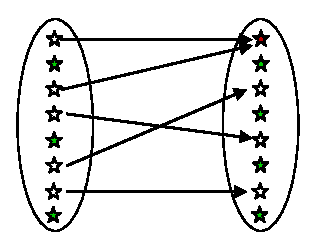
\includegraphics[width=4cm]{fonction} \\
\raisebox{-22mm}{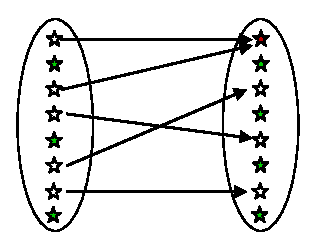
\includegraphics[height=2.5cm]{fonction.eps}} \\
\hline
Application\index{application}
&
Fonction définie partout:

\emph{\small (plus d'étoile verte dans~$E$)}

Une fonction~$f$ est une application si son ensemble de départ est égal à
son ensemble de définition.
&
%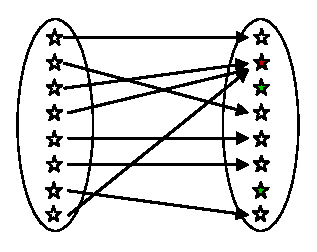
\includegraphics[width=4cm]{application} \\
\raisebox{-22mm}{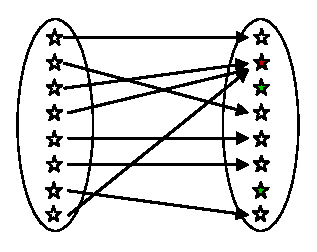
\includegraphics[height=2.5cm]{application.eps}} \\
\hline
Injection\index{injection}
&
Application telle que tout élément de~$F$ a au plus~$1$ antécédent.

$F$ a au moins autant d'éléments que~$E$.

\emph{\small (plus d'étoile verte dans~$E$ et plus d'étoile rouge dans~$F$)}

Soit~$\forall x,y\in \mathrm{e}^2, x\ne y \Rightarrow f(x)\ne f(y)$,

ou~$\forall x,y\in \mathrm{e}^2, f(x)=f(y) \Rightarrow x=y$
&
%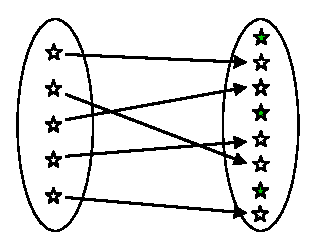
\includegraphics[width=4cm]{injection} \\
\raisebox{-22mm}{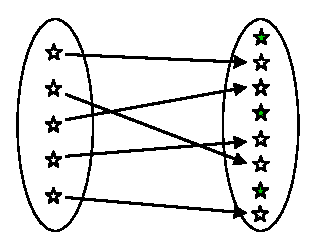
\includegraphics[height=2.5cm]{injection.eps}} \\
\hline
Surjection\index{surjection}
&
Application telle que tout élément de~$F$ a au moins~$1$ antécédent.

$F$ a au plus autant d'éléments que~$E$.

\emph{\small (plus d'étoile verte dans~$E$ et plus d'étoile verte dans~$F$)}

Soit~$\forall y\in F, \exists x\in E, f(x)=y$ , ou
$f$ est surjective si son ensemble image est égal à son ensemble d'arrivée.
&
%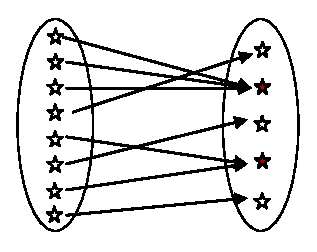
\includegraphics[width=4cm]{surjection} \\
\raisebox{-22mm}{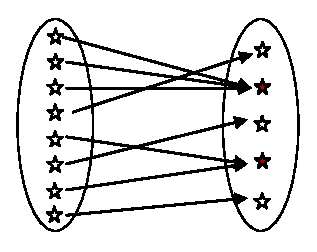
\includegraphics[height=2.5cm]{surjection.eps}} \\
\hline
Bijection\index{bijection}
&
C'est une injection ET une surjection:

chaque élément de l'ensemble de départ correspond à un seul élément de
l'ensemble d'arrivée et vice-versa.
&
%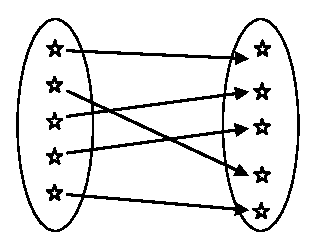
\includegraphics[width=4cm]{bijection} \\
\raisebox{-22mm}{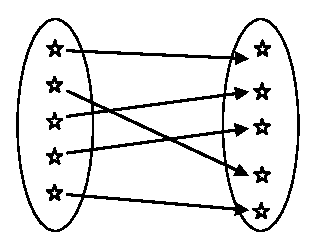
\includegraphics[height=2.5cm]{bijection.eps}} \\
\hline
\end{tabular}
\caption{{\protect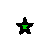
\includegraphics[width=1ex]{et-vert.eps}
= élément n'ayant pas de relation;
\protect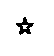
\includegraphics[width=1ex]{et-blanc.eps}
= élément ayant 1 relation;
\protect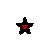
\includegraphics[width=1ex]{et-rouge.eps}
= élément ayant plus d'une relation.}}
\end{table}

Une étoile rouge dans~$E$ n'a pas de sens, cela voudrait dire qu'un élément de~$E$
peut avoir plusieurs valeurs différentes par la relation considérée...

\colorgris En fait, on sait donner un sens à cela. C'est ce que l'on appelle une
fonction multivaluée ou fonction multiforme ou fonction multivoque ou multifonction.
L'exemple le plus simple d'un fonction multiforme est la fonction réciproque d'une application
non injective (penser simplement aux fonctions circulaires).

On trouve les fonctions multiformes en analyse complexe: lorsque l'on veut utiliser le théorème des résidus
pour calculer une intégrale réelle, on peut être amené à considérer des restrictions (déterminations)
qui font de ces fonctions multiformes des fonctions (univoques), par exemple en utilisant la théorie des
revêtements qui considère des fonctions sur des surfaces de Riemann.\colorblack

\medskip
En restreignant une fonction à son domaine de définition, on en fait une application.
En la restreignant en plus à son ensemble d'arrivée on en fait une surjection
(une surjection, c'est un «truc» défini partout sur~$E$ et~$F$).

Quand on a une \underline{sur}jection, on est \underline{sûr} que tout élément
de l'ensemble de départ à une image, et que tout élément de l'ensemble
d'arrivée a un antécédent (au moins un même).

\colorgreen
Dans la pratique, on ne fait pas de distinction formelle entre fonction et application...

$f: \RR\to\RR, x\mapsto\sqrt{x}$ est une fonction, pas une application, car la racine carrée
n'est pas définie sur~$\RR$ mais sur~$\RR_+$.~$f: \RR_+\to\RR, x\mapsto\sqrt{x}$
est une application ! Mais pourquoi s'intéresserait-on à~$f$ là où elle n'est
pas définie... De plus, $f: \RR_+\to\RR_+, x\mapsto\sqrt{x}$ est une surjection
par définition (puisque l'on considère~$f$ de son ensemble de définition jusqu'à
son ensemble image). C'est évidemment une bijection (il ne reste que l'injectivité
à prouver...).\colorblack

\medskip
\begin{definition}[Support]
On appelle \textcolorblue{support}\index{support} d'une fonction~$f$ l'adhérence (ou la fermeture,
i.e. le plus petit fermé) du lieu où la fonction n'est pas nulle:
\begin{equation}\supp(f)=\overline{\{x\in\RR^n, f(x)\ne0\}}\end{equation}
\end{definition}

\medskip
\section{Morphismes}\index{morphisme}

\textcolorgris{Cette section est extraite du cours sur les structures algébriques. Nous l'avons toutefois sérieusement amputée pour coller à l'objectif de ce document.}

\medskip
\subsection{Présentation}

\begin{histoire}%
Mort au cours d'un duel à l'âge de vingt ans\index[aut]{Galois (Évariste), 1811-1832, Français}
 (ce qui en fait un héros romantique),
il laisse un manuscrit élaboré trois ans plus tôt, dans lequel il établit qu'une équation
algébrique est résoluble par radicaux si et seulement si le groupe de permutation de
ses racines a une certaine structure, qu'Emil Artin appellera justement résoluble.

\sbox{\MaBoiteAvecPhotos}{\setlength{\tabcolsep}{0pt}\scriptsize%
\begin{tabular}{c}%
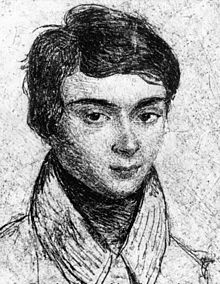
\includegraphics[height=\the\HauteurDesPhotos]{Galois}\\%
Galois%
\end{tabular}}
\medskip
\ImageADroite{%
Son Mémoire sur les conditions de résolubilité des équations par radicaux, publié par
Joseph Liouville quatorze ans après sa mort, a été considéré par ses successeurs,
en particulier Sophus Lie, comme le déclencheur du point de vue structural et méthodologique
des mathématiques modernes.\\
\indent
Toutefois, pour être tout à fait exact, Lagrange,\index[aut]{Lagrange (Joseph Louis, comte de -), 1736-1813, Italien}
reprenant une idée de d'Alembert\index[aut]{d'Alembert (Jean le Rond), 1717-1783, Français}
en vue de prouver qu'un polynôme de degré~$n$ possède
$n$ racines (i.e. que~$\CC$ est algébriquement clos), utilise des résultats sur les fonctions semblables
des racines, i.e. des fonctions rationnelles des racines qui restent invariantes par
les mêmes permutations. Ce résultat, qu'il a établi dans son fameux mémoire
de 1771 \emph{Réflexions sur la résolution algébrique}, inspirera Abel\index[aut]{Abel (Niels Henrik), 1802-1829, Norvégien}
et Galois\index[aut]{Galois (Évariste), 1811-1832, Français} et peut être
considéré comme le tout premier de la théorie des groupes.
}
\end{histoire}

\medskip
Soient deux ensembles~$G$ et~$G'$ munis d'un même type de
structure (topologique, groupe,
anneau, espace vectoriel, algèbre...).
Un \textcolorblue{morphisme (ou homomorphisme)} de~$G \to G'$ est une
\textcolorred{application~$f$ qui respecte cette structure.}

Pour ce faire, cette application doit vérifier certaines conditions, notamment une
certaine «linéarité» vis-à-vis des lois des~$G$ et~$G'$
(on pourrait également remplacer le terme linéarité par «capacité à faire
sortir de la fonction»).

\medskip
Un \textcolorblue{morphisme entre deux espaces topologiques} est tout simplement
une \textcolorred{application continue} (voir chapitre suivant sur la continuité).
C'est d'ailleurs ce dernier terme qui est utilisé en topologie, pas celui de morphisme (mais cela
revient bien au même).

\medskip
Un \textcolorblue{morphisme de groupe} entre~$(G,*)$ et~$(G',\star)$ satisfait à l'égalité suivante
qui est bien une \textcolorblue{«condition de linéarité par rapport à la loi»}:
$\colorred
\forall (x,y)\in G,\ f(x*y)=f(x)\star f(y)
$.
En particulier, si~$e$ et~$e'$ sont les éléments neutres de~$G$ et~$G'$, alors:~$f(e)=e'$.
Une autre conséquence directe est que:~$\forall x \in G,\ f(x^{-1})=[f(x)]^{-1}$.

\medskip
\subsection{Cas des espaces vectoriels: application et forme linéaires}\index{forme!linéaire}

\begin{definition}[Morphisme d'ev]
Soient~$(E,+,.)$ et~$(F,+,.)$ deux espaces vectoriels sur un corps~$\KK$.
Un \textcolorblue{morphisme d'ev}~$f$ entre~$E$ et~$F$ est une application qui respecte la condition
de linéarité par rapport aux lois~$+$ (en fait qui est un morphisme
de groupe entre les groupes~$(E,+)$ et~$(F,+)$) et qui conserve la
«linéarité par rapport à la multiplication par un scalaire»:
\begin{equation}\left\{
\begin{array}{ll}
\forall (x,y)\in \mathrm{e}^2, \quad f(x+ y)=f(x)+ f(y) &\text{ condition d'additivité}\\
\forall x\in E,\quad \forall \lambda\in\KK,\quad f(\lambda\cdot x)=\lambda\cdot f(x) &\text{ condition d'homogénéité}
\end{array}
\right.\end{equation}
\end{definition}

Ceci est équivalent à la condition suivante (on parle de «préservation des combinaisons
linéaires»):
\begin{equation}\colorred
\forall (x,y)\in \mathrm{e}^2,\quad \forall \lambda\in\KK,\quad f(\lambda\cdot x+ y)=\lambda \cdot f(x) + f(y)
\end{equation}
et on utilise plutôt le terme \textcolorblue{d'application linéaire} ou \textcolorblue{d'opérateur
linéaire} ou encore de \textcolorblue{transformation linéaire}.

\medskip
Dans le cas où~$F=\KK$, on ne parle pas d'application linéaire mais de \textcolorblue{forme linéaire}.
Une forme linéaire est donc une application linéaire définie sur~$E$ et à valeurs dans~$\KK$ (supposé
commutatif).
En d'autres termes, on parle de forme au lieu d'application, mais c'est la même chose !

\medskip
Si~$\varphi$ et~$\psi$ sont des formes linéaires et~$a$ et~$b$ des éléments de~$\KK$:
\begin{equation}
  \forall x \in E,\quad (a\varphi + b\psi)(x) = a\cdot \varphi(x) + b\cdot \psi(x)
\end{equation}

\medskip
L'application constante de valeur~$0_\KK$ s'appelle la «forme linéaire nulle».

\medskip
\subsection{Endo, iso, auto -morphismes}

Un \textcolorblue{endomorphisme}\index{morphisme!endomorphisme} est un morphisme d'une structure dans elle-même.

\medskip
Un \textcolorblue{isomorphisme} est est un morphisme~$f$ entre deux ensembles munis
de la même espèce de structure, tel qu'il existe un morphisme~$f'$ dans le sens inverse,
tels que~$f\circ f'$ et~$f'\circ f$ sont les identités des structures.
\textbff{Un isomorphisme est un morphisme bijectif.}

Deux ensembles munis du même type de structure algébrique sont dits \textcolorblue{isomorphes}
s'il existe un isomorphisme entre les deux ensembles.\index{morphisme!isomorphisme}

\textcolorred{L'isomorphie présente un intérêt majeur, car elle permet de transposer des résultats
et propriétés démontrés sur l'un des deux ensembles à l'autre.}

\medskip
Un \textcolorblue{automorphisme}\index{morphisme!automorphisme} est un isomorphisme d'une structure dans elle-même,
i.e. à la fois un isomorphisme et un endomorphisme.
\textbff{Un automorphisme est un endomorphisme bijectif.}

\medskip
L'identité d'un ensemble est toujours un automorphisme, quelle que soit la structure considérée.

\medskip
On note:
\begin{itemize}
  \item~$L_K(E,F)$ l'espace vectoriel des applications linéaires de~$E$ dans~$F$;
  \item~$\Isom_K(E,F)$ l'ensemble des isomorphismes de~$E$ dans~$F$;
  \item~$L_K(E)$ l'espace vectoriel des endomorphismes de~$E$;
  \item~$GL_K(E)$ le «groupe linéaire», i.e. le groupe des automorphismes de~$E$.
\end{itemize}

\medskip
\subsection{Espace dual d'un espace vectoriel}\index{dual d'un espace vectoriel}

\begin{definition}[Espace dual]
On appelle \textcolorblue{espace dual} d'un espace vectoriel~$E$ l'ensemble des
formes linéaires sur~$E$. Il est lui-même un~$\KK$-espace vectoriel, et on le note
$\mathrm{e}^*$ ou~$hom(E,\KK)$.
\end{definition}

La structure d'un espace et celle de son dual sont très liées.
Nous allons détailler quelques points en nous restreignant aux cas qui nous
intéressent (cas réel, dimension finie).

\medskip
\colorgris
Si l'on dispose, sur l'espace vectoriel considéré~$E$, d'un produit scalaire~$\langle\cdot,\cdot\rangle$ (voir
chapitre sur les espaces), alors il existe un moyen «naturel» de plonger~$E$ dans~$\mathrm{e}^*$ ,
i.e. d'associer à chaque élément de~$E$ un élément du dual, et ce de manière à
former un isomorphisme entre~$E$ et un sous-espace de~$\mathrm{e}^*$:
à chaque élément~$x\in E$ on associe la forme linéaire~$\varphi_x: E \to K;\ y \mapsto \langle x,y\rangle$.
Alors l'application~$f: E \to \mathrm{e}^*;\ x \mapsto \varphi_x$ est une application linéaire injective,
donc l'espace~$E$ est isomorphe au sous-espace~$f(E)$ de~$\mathrm{e}^*$.\colorblack

\medskip
\textcolorred{Si l'espace~$E$ est de dimension finie~$n$, alors l'espace dual~$\mathrm{e}^*$ est isomorphe à~$E$ et
est donc lui aussi de dimension~$n$.}
On a alors le théorème de la base duale (que je ne présente pas, car je n'ai pas
parlé de base... mais peut-être pourrons-nous nous passer de ces rappels dans ce
document).

\medskip
Pour~$x \in E$, on note~$\langle\varphi,x\rangle$ pour~$\varphi(x)$.
Cette notation est appelée \textcolorblue{crochet de dualité.}\index{crochet de dualité}

\medskip
\begin{definition}[Dual topologique]\index{dual topologique d'un espace vectoriel}
Soit~$E$ un espace vectoriel topologique sur le corps~$\KK$.
Le dual topologique~$E'$ de~$E$ est le sous-espace vectoriel de~$\mathrm{e}^*$ (le dual algébrique de~$E$)
formé des formes linéaires continues.
\end{definition}
Si l'espace est de dimension finie, le dual topologique coïncide avec le dual algébrique,
puisque dans ce cas toute forme linéaire est continue.
Mais dans le cas général, l'inclusion du dual topologique dans le dual algébrique est stricte.
%\colorblack

\medskip
\subsection{Noyau et image}\index{noyau}\index{image}

\begin{definition}[Noyau]
Le \textcolorblue{noyau} du morphisme~$f$ est l'ensemble des antécédents de l'élément neutre:
\begin{equation} \ker(f)=\left\{x\in E, f(x)=0\right\}=f^{-1}(\{0\})\end{equation}
\end{definition}
et \textcolorgreen{$f$ est injectif si et seulement si son noyau est réduit à~$\{0\}$.}

\medskip
\begin{definition}[Image]
L'\textcolorblue{image} du morphisme~$f$ est l'image par~$f$ de~$E$:
\begin{equation} \operatorname{im}(f)=\left\{ f(x), x\in E\right\}=f(E)\end{equation}
\end{definition}
et \textcolorgreen{$f$ est surjectif si et seulement si son image est égale à~$F$.}

\medskip
Dans le cas d'\textbff{espaces vectoriels},
l'ensemble~$\ker(f)$ est un sous-espace vectoriel de~$E$ et
l'ensemble~$\operatorname{im}(f)$ est un sous-espace vectoriel de~$F$.

\begin{theoreme}[Théorème du rang]
Il est assez visible que (théorème de factorisation)~$f$ induit un isomorphisme de
l'espace vectoriel quotient~$E/\ker(f)$ sur l'image~$\operatorname{im}(f)$.
Deux espaces isomorphes ayant même dimension, il s'en suit la relation,
valable pour un espace~$E$ de dimension finie, appelée théorème du rang:\index{théorème!du rang}
\begin{equation}
  \dim(\ker(f)) + \dim(\operatorname{im}(f)) = \dim( E )
\end{equation}
Le nombre~$\dim(\operatorname{im}(f))$ est aussi appelé rang de~$f$ et est noté
$\operatorname{rg}(f)$.
\end{theoreme}

On a également:
\begin{itemize}
  \item l'image réciproque d'un sous-espace vectoriel de~$F$ par~$f$ est un sous-espace vectoriel de~$E$;
  \item l'image directe d'un sous-espace vectoriel de~$E$ par~$f$ est un sous-espace vectoriel de~$F$.
\end{itemize}

\medskip
\section{Opérateur}\index{opérateur}

Le terme «opérateur» a été utilisé au paragraphe précédent... regardons d'un peu
plus près.

\medskip
D'une manière générale, un \textcolorblue{opérateur} est une application entre
deux espaces vectoriels topologiques.

\medskip
Un opérateur~$O: E \to F$ est \textcolorblue{linéaire} si et seulement si:
\begin{equation}\forall (\lambda, \mu) \in \KK^2,\quad\forall (x_1, x_2) \in E,\quad O( \lambda x_1 + \mu x_2)=\lambda O(x_1) + \mu O(x_2)
\end{equation}
où~$\KK$ est le corps des scalaires de~$E$ et~$F$.

\medskip
\textcolorred{Lorsque~$F = \RR$, un opérateur est une fonctionnelle sur~$E$.}

\medskip
Un opérateur est \textcolorblue{continu} s'il est continu en tant qu'application (pour la définition de la
continuité, voir chapitre suivant.


\medskip
Un \textcolorblue{opérateur différentiel} est un opérateur agissant sur des
fonctions différentiables au sens des dérivés ordinaires ou partielles: voir définition
au chapitre suivant.

\medskip
On définit également les opérateurs différentiels elliptiques et hyperboliques.
Mais pour cela, il faut introduire les notions de symbole et symbole principale d'un
opérateur... et cela ne nous semble ni adapté à ce document, ni suffisamment
«naturel» pour cet exposé.
\textcolorgreen{Nous nous contenterons de définir plus loin les notions
d'équations aux dérivées partielles linéaires et homogènes du second-ordre dites elliptiques, hyperboliques
et paraboliques.}




%\medskip
%\section{Réduction des endomorphismes}
%
%\textcolorgris{Le sujet a été traité en long, en large et en travers en taupe, nous
%ne faisons que rappeler l'essentiel.}
%
%\medskip
%Une fois que l'on a remarqué qu'un endomorphisme peut s'écrire sous forme matricielle,
%la réduction d'endomorphisme consiste à exprimer un endomorphisme sous une forme
%plus simple en trouvant une nouvelle base de l'espace vectoriel.
%
%\medskip
%Bien qu'une réduction \textcolorred{ne soit pas unique}, elle doit néanmoins satisfaire aux points
%suivants:
%\begin{itemize}
%  \item L'endomorphisme définit par restriction un nouvel endomorphisme sur chacun
%	des sous-espaces (i.e. chacun est un sous-espace vectoriel stable), ainsi la petite
%	structure est une entité intrinsèque avec sa propre cohérence;
%  \item Les différents sous-espaces sont en somme directe, i.e. indépendants les uns des autres.
%  \item Les différents sous-espaces engendrent l'espace entier (ils sont supplémentaires),
%	ce qui offre l'exhaustivité de l'analyse.
%  \item La réduction décrit l'intégralité de la structure originelle.
%  \item Elle est maximale, i.e. qu'il n'existe pas de décomposition en éléments plus petits
%	et donc plus simple.
%  \item Elle est aussi simple que possible, i.e. que pour chacune des sous-structures il n'existe
%	pas de représentation plus élémentaire.
%\end{itemize}
%
%
%\medskip
%\section{Valeurs propres, spectre}
% 